% CVPR 2026 Paper Template; see https://github.com/cvpr-org/author-kit

\documentclass[10pt,twocolumn,letterpaper]{article}

%TODO: CAMERA-READY
%%%%%%%%% PAPER TYPE  - PLEASE UPDATE FOR FINAL VERSION
%\usepackage{cvpr}              % To produce the CAMERA-READY version
%\usepackage[review]{cvpr}      % To produce the REVIEW version
\usepackage[pagenumbers]{cvpr} % To force page numbers, e.g. for an arXiv version

% Import additional packages in the preamble file, before hyperref
\input{preamble}

% It is strongly recommended to use hyperref, especially for the review version.
% hyperref with option pagebackref eases the reviewers' job.
% Please disable hyperref *only* if you encounter grave issues, 
% e.g. with the file validation for the camera-ready version.
%
% If you comment hyperref and then uncomment it, you should delete *.aux before re-running LaTeX.
% (Or just hit 'q' on the first LaTeX run, let it finish, and you should be clear).
\definecolor{cvprblue}{rgb}{0.21,0.49,0.74}
\usepackage[pagebackref,breaklinks,colorlinks,allcolors=cvprblue]{hyperref}

%%%%%%%%% PAPER ID  - PLEASE UPDATE
\def\paperID{*****} % *** Enter the Paper ID here
\def\confName{CVPR}
\def\confYear{2026}

%%%%%%%%% TITLE - PLEASE UPDATE
\title{MOO: A Multi-view Oriented Observations Dataset for Viewpoint Analysis in Cattle Re-Identification}

%%%%%%%%% AUTHORS - PLEASE UPDATE
\author{
William Grolleau$^{1*}$
Achraf Chaouch$^{1}$
Astrid Sabourin$^{1}$
Guillaume Lapouge$^{1*}$
Catherine Achard$^{2}$ \\
\\
{\small $^1$Universite Paris-Saclay, CEA, List, F-91120 Palaiseau, France} \\
{\small $^2$Sorbonne University, CNRS, ISIR, 4 Place Jussieu, 75005 Paris, France} \\
{\texttt{\small \{william.grolleau, guillaume.lapouge\}@cea.fr}} \\
Project page: \url{https://github.com/TurtleSmoke/MOO}
}

\begin{document}
    \maketitle
    \begin{abstract}
    Animal re-identification (ReID) faces critical challenges due to viewpoint variations, particularly in Aerial-Ground (AG-ReID) settings where models must match individuals across drastic elevation changes.
    However, existing datasets lack the precise angular annotations required to systematically analyze these geometric variations.

    To address this, we introduce the \textbf{M}ulti-view \textbf{O}riented \textbf{O}bservation (MOO) dataset, a large-scale synthetic AG-ReID dataset of $1,000$ cattle individuals captured from $128$ uniformly sampled viewpoints ($128,000$ annotated images).

    Using this controlled dataset, we quantify the influence of elevation and identify a critical elevation threshold, above which models generalize significantly better to unseen views.

    Finally, we validate the transferability to real-world applications in both zero-shot and supervised settings, demonstrating performance gains across four real-world cattle datasets and confirming that synthetic geometric priors effectively bridge the domain gap.
    Collectively, this dataset and analysis lay the foundation for future model development in cross-view animal ReID.

    MOO is publicly available at \url{https://github.com/TurtleSmoke/MOO}.
\end{abstract}
    \section{Introduction}
\label{sec:introduction}

Animal Re-identification (ReID) aims to recognize and match a specific individual across different non-overlapping camera views, despite variations in pose or viewpoint.
It is an essential component for automated tracking in wildlife conservation and livestock management.

However, in real-world deployments, camera placement is often constrained by physical limitations in closed spaces or wild environments.
This is particularly challenging in Aerial-Ground ReID (AG-ReID) scenarios, where models must associate individuals across drastic perspective changes.
Identifying which viewpoints maximize identification accuracy is therefore crucial for optimizing sensor placement configurations.

While viewpoint dependencies have been extensively studied in human ReID~\cite{sunDissectingPersonReIdentification2019a}, equivalent insights for animals remain lacking.
This gap is detrimental, as animals often exhibit asymmetric coat patterns, making their identification highly sensitive to viewpoint shifts.
Existing datasets lack precise angular annotations and cannot perform systematic analysis of viewpoint impact.

To bridge this gap, we introduce the \textbf{M}ulti-view \textbf{O}riented \textbf{O}bservation (MOO), a large-scale synthetic AG-ReID dataset.
MOO contains 1,000 synthetic cattle identities rendered from 128 uniformly sampled viewpoints spanning $360^\circ$ in azimuth and $-25^\circ$ to $90^\circ$ elevation (relative to the horizontal side view).
By isolating identity through asymmetric patterns, we systematically analyze viewpoint sensitivity.
Ultimately, this work lays the foundation for future model development on geometric robustness in animal ReID.

Our contributions are threefold:
\begin{itemize}
    \item We present the MOO dataset, a large-scale synthetic benchmark for patterned animal ReID with precise azimuth and elevation annotations.
    \item We provide the first systematic quantification of elevation impact on patterned animal ReID, identifying a $30^\circ$ elevation angle as a key threshold for generalization.
    \item We demonstrate that MOO serves as a robust pre-training source, yielding consistent performance gains on real-world datasets in both zero-shot and supervised scenarios.
\end{itemize}

\begin{figure*}[tbp]
    \centering
    
\includegraphics[width=1.0\linewidth]{gabstract}
    \caption{MOO: A synthetic dataset for systematic analysis and real-world transferability. The workflow encompasses (1) individual generation; (2) dataset rendering; and (3) systematic analysis and real-world transfer.}
    \label{fig:gabstract}
\end{figure*}

    \section{Related work}
\label{sec:related_work}

\subsection{Dataset Limitations}

Agricultural datasets typically restrict observations to fixed top-down~\cite{andrewVisualIdentificationIndividual2021a, gaoSelfSupervisionVideoIdentification2021b, xiaoCowIdentificationFreestall2022b, yuMultiCamCows2024MultiviewImage2024} or lateral~\cite{zhaoCompactLossVisual2022, liIndividualDairyCow2021} perspectives.
While some approaches focus on discriminative anatomical regions~\cite{adamSeaTurtleID2022LongspanDataset2024a, shojaeipourAutomatedMuzzleDetection2021, moskvyakLearningLandmarkGuided2020} or combine multiple static views~\cite{bergaminiMultiviewsEmbeddingCattle2018a, li2024cattle}, they lack the continuous viewpoint coverage required for geometric analysis.

In contrast, wildlife datasets~\cite{liATRWBenchmarkAmur2020, parham2017animal, atanbori2024spots, nepovinnykhSealIDSaimaaRinged2022a, dlaminiAutomatedIdentificationIndividuals2020b} offer larger viewpoint diversity but suffer from uncontrolled environments.
In these scenarios, the absence of precise annotations and the presence of occlusion or background clutter make it difficult to decouple viewpoint effects from environmental bias.

Synthetic data, while used for pose~\cite{Jiang2022BMVC, bonettoZebraPoseZebraDetection2024} or segmentation~\cite{muLearningSyntheticAnimals2020a, pengLearningPartSegmentation2024}, remains underutilized in ReID, with existing examples lacking precise viewpoint labels~\cite{picekCzechLynxDatasetIndividual2025}.

As highlighted in \Cref{tab:dataset metrics}, MOO addresses these limitations by combining controlled diversity with precise geometric metadata.

\begin{table*}[tbp]
    \centering
    \caption{
        Comparison of wildlife and cattle re-identification datasets with MOO.
        \textit{Non-Correlated Images}: independent frames reducing temporal and background bias.
        \textit{Synthetic}: includes synthetic data.
        \textit{Annotation}: viewpoint labels provided as continuous angles (Az./El.) or discrete categories.
    }
    \label{tab:dataset metrics}

    \scriptsize

    \begin{tabular}{llrrlccc}
        \toprule

        \textbf{Species}
        & \textbf{Dataset}
        & \textbf{Individuals}
        & \textbf{Images}
        & \textbf{View}
        & \textbf{Synthetic}
        & \textbf{Non-Correlated Images}
        & \textbf{Annotation} \\

        \midrule
        \multirow{6}{*}{Wildlife}

        & ATRW~\cite{liATRWBenchmarkAmur2020}
        & 107 & 3,649 & Lateral & $\circ$ & $\bullet$ & \\

        & SealID~\cite{nepovinnykhSealIDSaimaaRinged2022a}
        & 57 & 2,080 & Lateral & $\circ$ & $\bullet$ & \\

        & SeaTurtleIDHeads~\cite{adamSeaTurtleID2022LongspanDataset2024a}
        & 438 & 8,729 & Lateral & $\circ$ & $\bullet$ & \\

        & Nyala Data~\cite{dlaminiAutomatedIdentificationIndividuals2020b}
        & 237 & 1,942 & Lateral & $\circ$ & $\bullet$ & Left vs Right \\

        & LeopardID~\cite{atanbori2024spots}
        & 430 & 6,805 & Lateral & $\circ$ & $\bullet$ & \\

        & CzechLynx~\cite{picekCzechLynxDatasetIndividual2025}
        & 219+300 & 37k+100k & Lateral & $\bullet$ & $\bullet$ & \\

        \midrule
        \multirow{10}{*}{Cattle}

        & Multi-views Embedding~\cite{bergaminiMultiviewsEmbeddingCattle2018a}
        & 439 & 17,802 & Lateral & $\circ$ & $\circ$ & Front vs Side \\

        & OpenCows2020~\cite{andrewVisualIdentificationIndividual2021a}
        & 46 & 4,736 & Top & $\circ$ & $\circ$ & \\

        & Cows2021~\cite{gaoSelfSupervisionVideoIdentification2021b}
        & 182 & 13,784 & Top & $\circ$ & $\circ$ & \\

        & MuzzleCows~\cite{shojaeipourAutomatedMuzzleDetection2021}
        & 300 & 2,900 & Face & $\circ$ & $\bullet$ & \\

        & Dairy Cows 2021~\cite{liIndividualDairyCow2021}
        & 13 & 1,485 & Lateral & $\circ$ & $\bullet$ & \\

        & MVCAID100~\cite{zhaoCompactLossVisual2022}
        & 100 & 4,073 & Lateral & $\circ$ & $\circ$ & \\

        & Cows Stall Barn~\cite{xiaoCowIdentificationFreestall2022b}
        & 48 & 8,640 & Top & $\circ$ & $\circ$ & \\

        & MultiCamCows2024~\cite{yuMultiCamCows2024MultiviewImage2024}
        & 90 & 101,329 & Top & $\circ$ & $\circ$ & \\

        & CoBRA ReID~\cite{perneelDynamicMultiBehaviourOrientationInvariant2025}
        & 48 & 11,438 & Top & $\circ$ & $\circ$ & Az. Angle \\

        & \textbf{MOO}
        & \textbf{1000} & \textbf{128,000} & \textbf{All} & $\bullet$ & $\bullet$ & \textbf{Az. \& El. Angle} \\

        \bottomrule
    \end{tabular}
\end{table*}

\subsection{Viewpoint-Agnostic ReID}
\label{subsec:viewpoint-agnostic-reid}
Viewpoint change is a fundamental challenge in patterned animal ReID, as it deeply influences the perception of discriminative features.

To achieve view-invariance, approaches range from deep metric learning~\cite{zhaoCompactLossVisual2022, zhaoMultiCenterAgentLoss2022} and local descriptor alignment~\cite{chenHolsteinCattleFace2022b} to explicitly targeting discriminative body regions~\cite{shojaeipourAutomatedMuzzleDetection2021, nepovinnykhReidentificationPatternedAnimals2025c, phyoHybridRollingSkew2018, dacLivestockIdentificationUsing2022, nepovinnykhSpeciesAgnosticPatternedAnimal2024}.
Other works attempt to resolve geometric ambiguity by unwrapping 3D textures into normalized 2D maps~\cite{hiby2009tiger, algasovUnsupervisedPelagePattern2025} or employing multi-branch networks to jointly learn from multiple views~\cite{bergaminiMultiviewsEmbeddingCattle2018a, li2024cattle}.

However, unlike human ReID~\cite{sunDissectingPersonReIdentification2019a}, the animal domain lacks a fundamental quantification of how specific angular changes degrade feature perception.
We provide this foundational analysis to guide future model development.

In this work, we conduct a systematic study of the impact of viewpoint variations on patterned animals and lay the foundation for developing more robust models for real-world applications.

    \section{Dataset description}
\label{sec:dataset_description}
\subsection{Generation Pipeline}
\label{subsec:generation-pipeline}

We utilize a realistic \href{https://www.turbosquid.com/3d-models/cow-3d-model/1126261}{3D cow mesh} in a neutral pose.
To ensure diversity, we generate unique identities based on a \href{https://github.com/CorentinDumery/cow-tex-generator}{procedural texture generation} applied on the mesh via UV mapping as illustrated in \Cref{fig:gabstract}.
Images are rendered with foreground masks to eliminate background bias, a known issue in ReID~\cite{picekAnimalIdentificationIndependent2024a,tianEliminatingBackgroundbiasRobust2018, yuAddressingElephantRoom2024}.
The virtual camera samples viewpoints based on a uniform grid of $16$ azimuths ($\phi \in [0^\circ, 360^\circ)$) and $8$ elevations ($\theta \in [0^\circ, 85^\circ]$), with random jitters ($\pm{10}^\circ$ and $\pm{5}^\circ$, respectively) added to simulate continuous variations and prevent grid overfitting.
All images are rendered using Blender at a resolution of $512 \times 512$ pixels, resulting in a total of $128,000$ images for the $1,000$ identities.

\subsection{Metadata}
\label{subsec:metadata}

Beyond RGB images, the dataset provides comprehensive annotations for each image.
This includes angular information ($\phi, \theta$), camera calibration, and labels.
To improve geometric tasks, we also provide depth maps rendered from the same viewpoints as the RGB images.

\subsection{Evaluation Protocols}
\label{subsec:eval_prot}

We partition the dataset equally into training and testing sets, with $500$ identities per set.
To simulate realistic monitoring scenarios, images captured below $30^\circ$ are classified as side views, while images above $30^\circ$ are classified as top views.

We establish three training configurations: Side-only, Top-only, and Top-Side.
Similarly to AG-ReID scenarios, we define three evaluation protocols with query $\rightarrow$ gallery being: Top $\rightarrow$ Side, Side $\rightarrow$ Top, and Top-Side $\rightarrow$ Top-Side.


    \section{Viewpoint Analysis}
\label{sec:viewpoint_analysis}

\subsection{Implementation Details}
\label{subsec:implementation-details}

We train a baseline on MOO using an ImageNet-21k~\cite{ridnikImageNet21KPretrainingMasses2021a} pre-trained ViT backbone~\cite{dosovitskiyImageWorth16x162020a} paired with a fully connected classification head.
Following standard ReID practices~\cite{9025455}, images are resized to 256x256 pixels, and augmented with random cropping and horizontal flipping.
The model is trained for 120 epochs using a batch size of 128 (4 images per ID).
We use an SGD optimizer (momentum 0.9, weight decay 1e-4) with a base learning rate of 0.008 and cosine decay, jointly optimizing cross-entropy and triplet losses to constrain the feature space~\cite{9025455}.
We use mean Average Precision (mAP) and Rank-1 accuracy as evaluation metrics, computed using the standard Cumulative Matching Characteristic (CMC) curve.

\subsection{Elevation Impact}
\label{subsec:elevation_impact}

To systematically quantify the impact of viewpoint, we partitioned the dataset into 8 elevation levels ($\theta \in [0^\circ, 85^\circ]$) and 4 azimuthal views (Right, Front, Left, Back) based on our generation grid introduced in section~\ref{subsec:generation-pipeline}.

\subsubsection*{Single-View training}

\Cref{fig:elev1} shows the performance of models trained on a single elevation partition (for query and gallery) and evaluated against all other elevations, in a same-view setup (\ie query and gallery images are drawn from the same partition)

While each model performs best on the partition it was trained on, we observe a distinct asymmetric degradation: models trained at higher elevations generalize significantly better to lower views than vice versa.
Specifically, elevations superior to $30^\circ$ enable robust ReID.
This suggests that, beyond this elevation, top-down views preserve enough shared features across azimuth changes, whereas side views suffer from self-occlusion.

\begin{figure}[tbp]
    \centering
    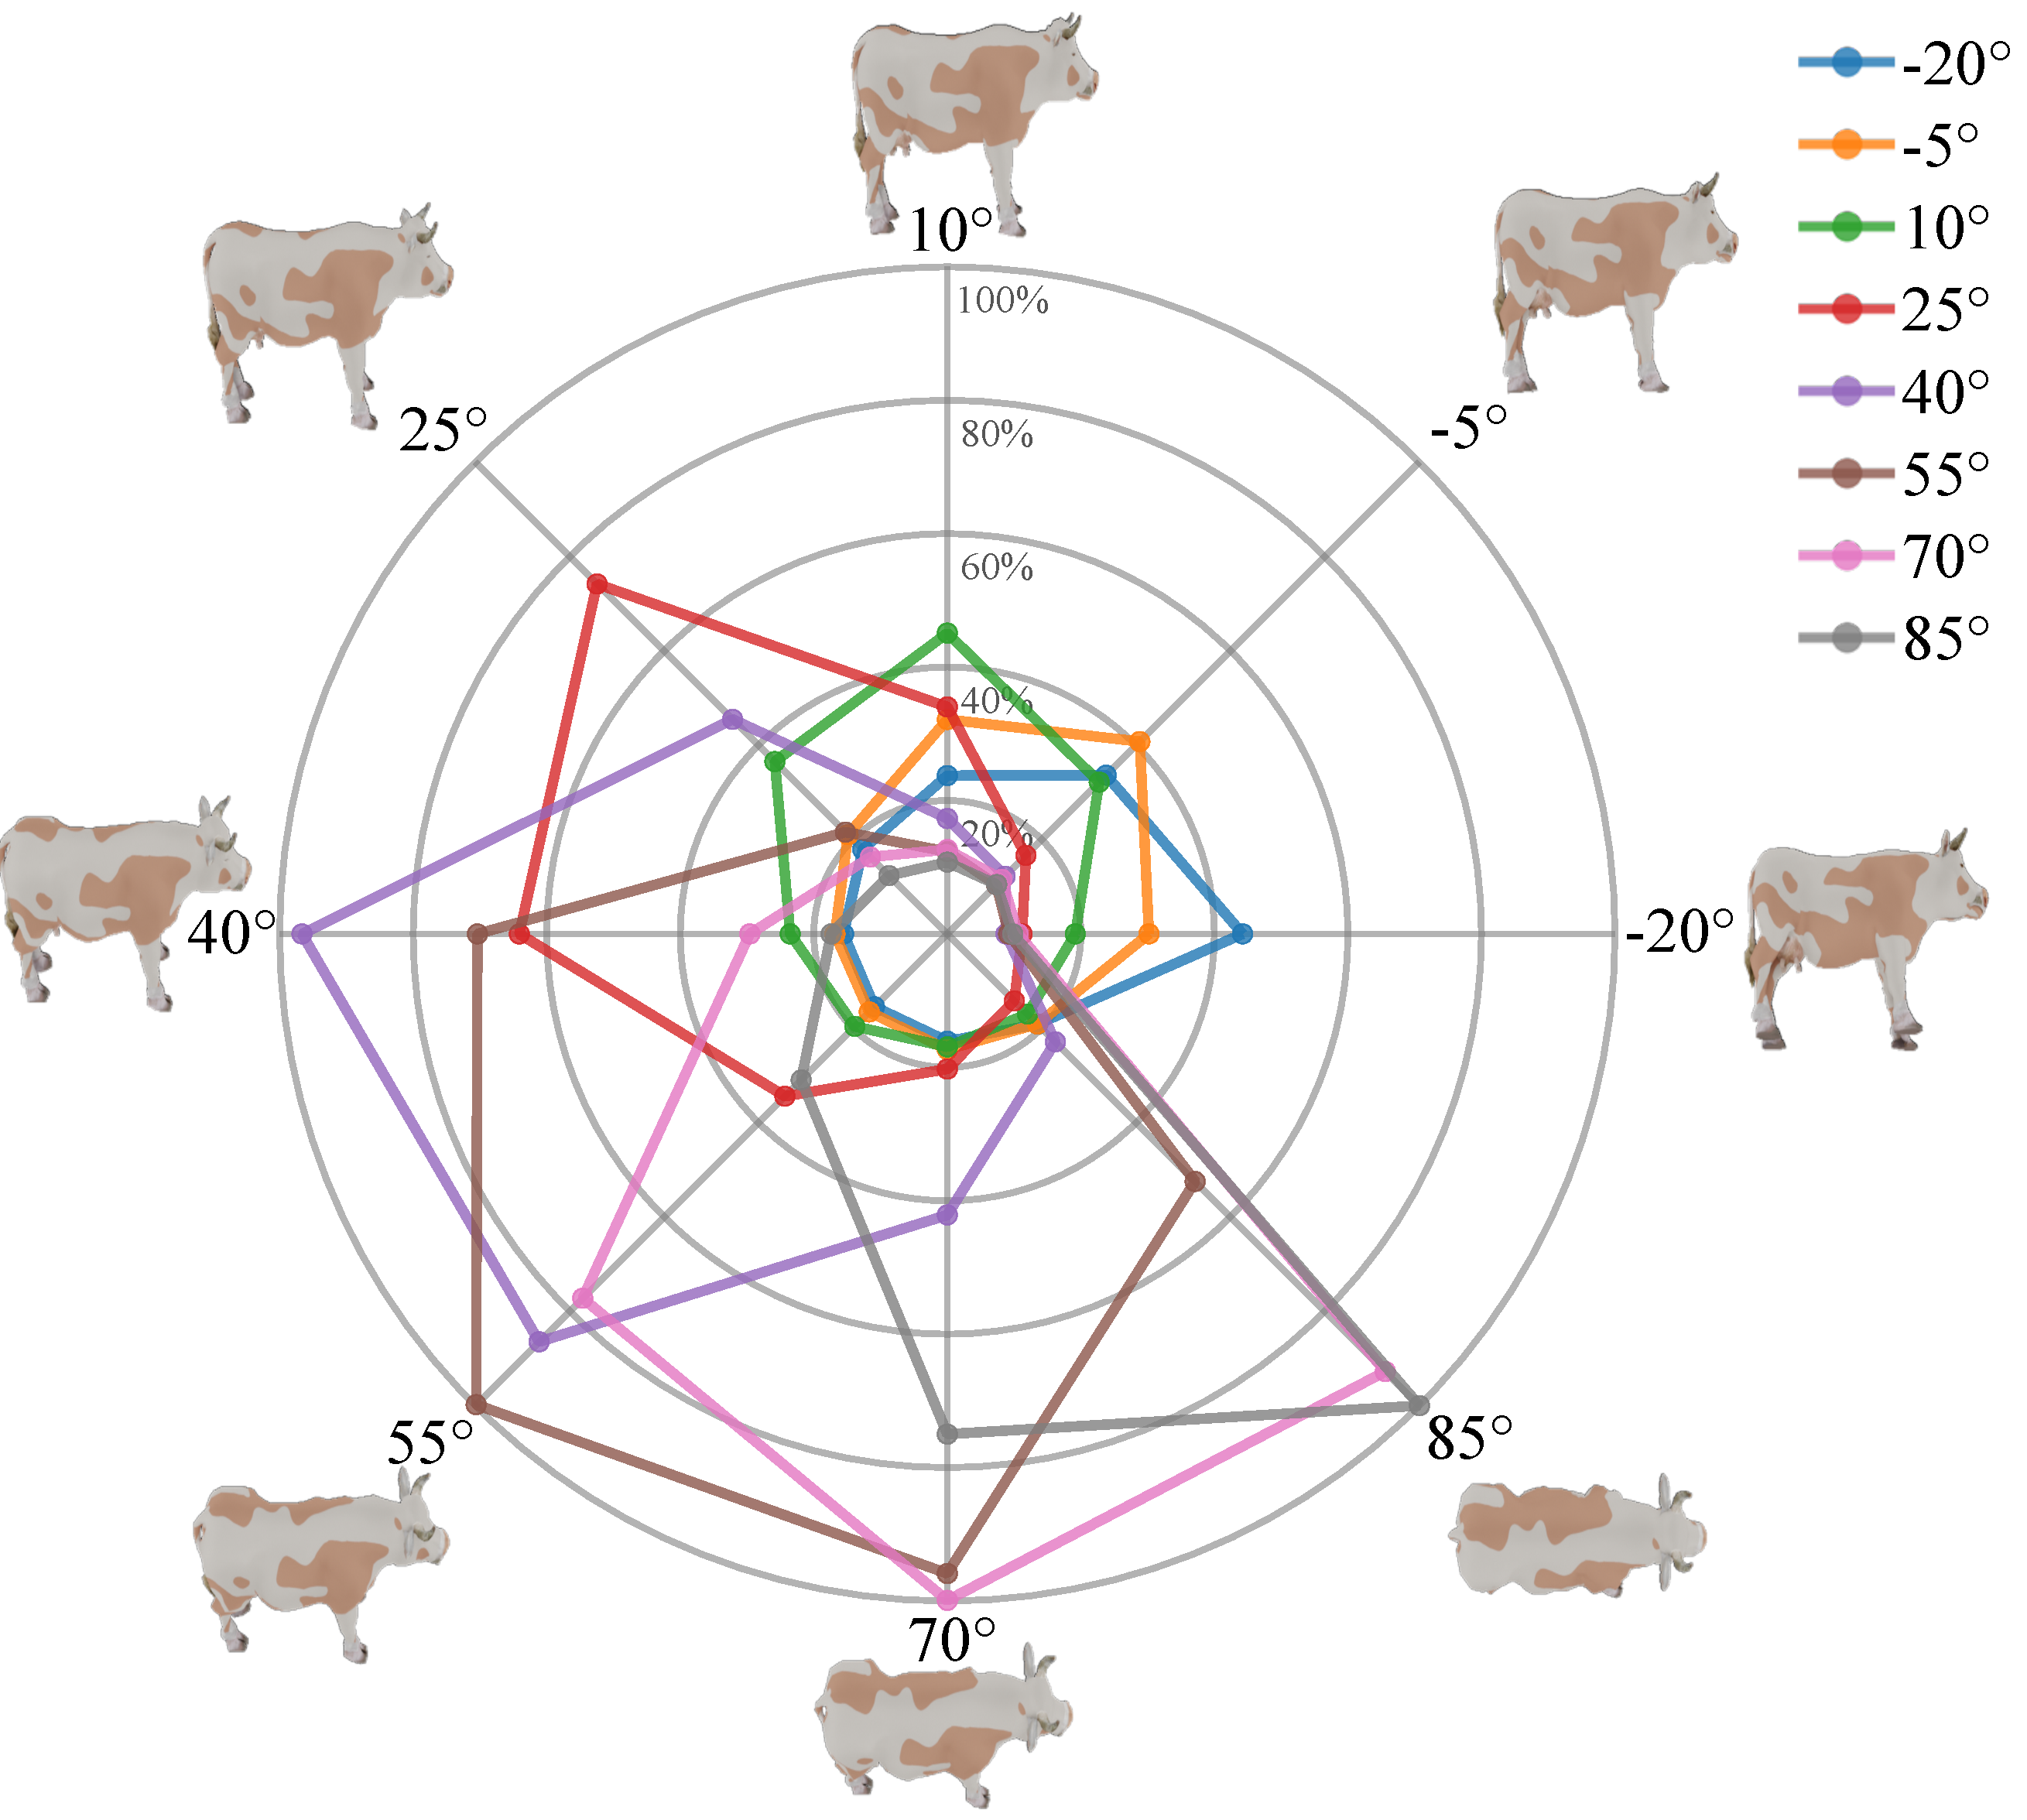
\includegraphics[width=1.0\linewidth]{figure_4}
    \caption{mAP per training elevation range across eight partitions evaluated in a same-view setup, where Query and gallery images share the same elevation.}
    \label{fig:elev1}
\end{figure}

\subsubsection*{All-View training}

We further investigated whether increasing elevation diversity during training improves generalization.
As shown in \Cref{fig:elev2}, training on broader consistently falls short of the theoretical upper bound set by view-specific experts (black dot).
This inability to match specialized models suggests that simply scaling data is insufficient.

\begin{figure}[tbp]
    \centering
    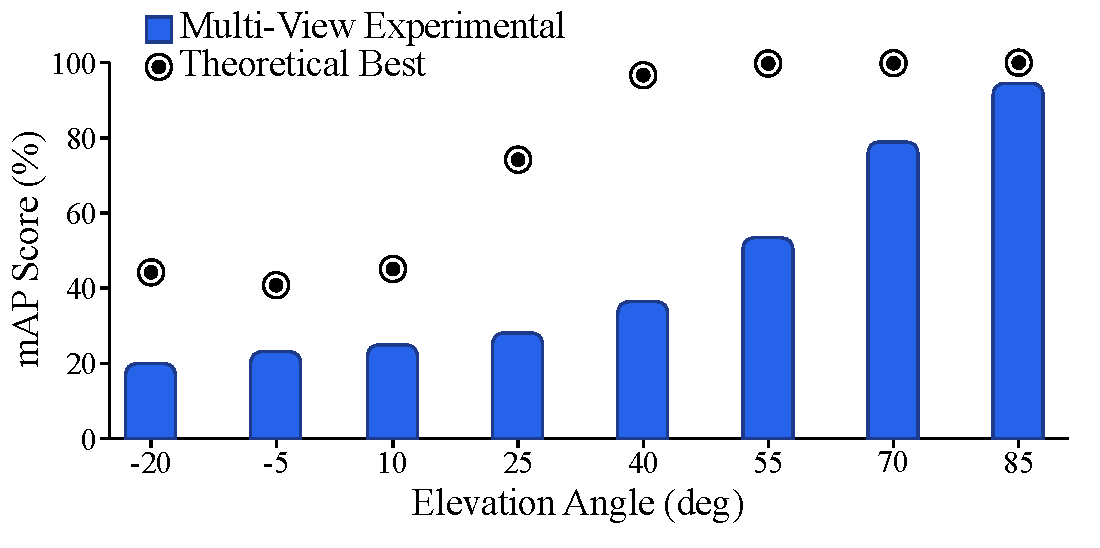
\includegraphics[width=1.0\linewidth]{expert}
    \caption{
        mAP for the best Single-View expert (black dot) and All-View model (blue curve) across eight partitions evaluated in a same-view setup, where Query and gallery images share the same elevation.
    }
    \label{fig:elev2}
\end{figure}

\subsection{Azimuth Impact}
\label{subsec:azimuth-impact}

\Cref{tab:azimuth} demonstrates a clear performance gap where training on lateral views (Right/Left) achieve near-perfect accuracy ($>0.98$), whereas sagittal views (Front/Back) are significantly more challenging.
Naturally, matching the training and inference views yields the best results, but on average, lateral views still outperform sagittal views by $20\%$ mAP and should be prioritized for camera placement when possible.

\begin{table}[t]
    \centering
    \caption{
        mAP across four azimuth training and evaluation scenarios evaluated in a same-view setup, where Query and gallery images share the same view.
    }
    \label{tab:azimuth}

    \scriptsize

    \begin{tabular}{lccccc}
        \toprule
        \diagbox{\textbf{Train}}{\textbf{Test}} & Right         & Left          & Front         & Back          & Average       \\
        \midrule
        Right                                   & \textbf{0.98} & 0.99          & 0.16          & 0.15          & 0.63          \\
        Left                                    & 0.99          & \textbf{0.99} & 0.17          & 0.16          & \textbf{0.65} \\
        Front                                   & 0.42          & 0.42          & \textbf{0.56} & 0.24          & 0.40          \\
        Back                                    & 0.50          & 0.51          & 0.29          & \textbf{0.75} & 0.48          \\
        \bottomrule
    \end{tabular}
\end{table}

    \section{Experiments}
\label{sec:experiments}

\subsection{MOO Benchmark}
\label{subsec:_benchmark}

We evaluate MOO under AG-ReID scenarios in \Cref{tab:benchmark}.
Despite the controlled synthetic environment, the task remains highly challenging: the upper bound (supervised on Top-Side) reaches only $52.5\%$ mAP, far from saturation.
Furthermore, cross-view generalization is difficult.
In the \textbf{Side $\to$ Top} scenario, performance drops from $41.6\%$ (using all views) to just $13.0\%$ when trained on Side views only, and $25.0\%$ when trained on Top views only.

\begin{table}[tbp]
    \centering
    \caption{
        mAP and Rank-1 comparison for three training configurations across three evaluation (query $\rightarrow$ gallery) scenarios.
    }
    \label{tab:benchmark}

    \scriptsize

    \begin{tabular}{l cc cc cc}
        \toprule

        & \multicolumn{2}{c}{\textbf{Top $\rightarrow$ Side}}
        & \multicolumn{2}{c}{\textbf{Side $\rightarrow$ Top}}
        & \multicolumn{2}{c}{\textbf{Top-Side $\rightarrow$ Top-Side}} \\

        \cmidrule(lr){2-3} \cmidrule(lr){4-5} \cmidrule(lr){6-7}

        \textbf{Training}
        & \textbf{mAP} & \textbf{R-1}
        & \textbf{mAP} & \textbf{R-1}
        & \textbf{~~~~mAP} & \textbf{R-1} \\

        \midrule

        Train Side
        & 13.1 & 35.6
        & 13.0 & 75.5
        & ~~~~20.6 & 97.4 \\

        Train Top
        & 22.0 & 94.7
        & 25.0 & 29.7
        & ~~~~39.4 & 87.2 \\

        Train Top-Side
        & \textbf{39.4} & \textbf{96.2}
        & \textbf{41.6} & \textbf{79.7}
        & ~~~~\textbf{52.5} & \textbf{99.7} \\

        \bottomrule
    \end{tabular}
\end{table}

\subsection{Real-World Transferability}
\label{subsec:real_world_transfer}

We evaluate MOO's transferability on four real-world datasets: FriesianCattle2015 (FC15)~\cite{andrewAutomaticIndividualHolstein2016}, FriesianCattle2017 (FC17) and AerialCattle2017 (AC17)~\cite{andrewVisualLocalisationIndividual2017}, and Cows2021 (C21)~\cite{gaoSelfSupervisionVideoIdentification2021b}.
We assess the benefit of transferring geometric priors by comparing a standard ImageNet-21k baseline against models that undergo additional pre-training on MOO (using either All views or Top views only).

In the zero-shot setup (\Cref{tab:real}), adding MOO pre-training consistently outperforms the ImageNet-21k baseline.
%Notably, adding a pre-training solely on \textbf{MOO Top-views} often yields superior results than using the full dataset.
For example, on Cows21 (a top-down dataset), MOO Top-view pre-training achieves $32.1\%$ mAP zero-shot, compared to $13.4\%$ with All-views and $9.4\%$ with the baseline.
This underscores the value of MOO's annotations: they allow for strategic selection of training data.

In the supervised setup, the ImageNet-21k + MOO initialization improves performance on all datasets except FriesianCattle2017.
This could be attributed to confounding factors in this dataset, such as multiple cows per frame, occlusions, and complex backgrounds. %, which may diminish the benefits of MOO's geometric priors.
Overall, these results confirm MOO's practical relevance, providing features that generalize effectively to real images.
%Overall, these results confirm MOO's practical relevance, providing features that generalize effectively to real images and that viewpoint control during training maximizes real-world performance.

\begin{table}[t]
    \centering
    \caption{
        Transfer learning results on four real-world datasets.
        We compare the standard ImageNet baseline with our pre-training on MOO.
        \textbf{Top:} Zero-shot evaluation.
        \textbf{Bottom:} Supervised training on the target dataset.
    }
    \label{tab:real}

    \scriptsize
    \setlength{\tabcolsep}{2pt}

    \begin{tabular}{l cc cc cc cc}
        \toprule

        & \multicolumn{2}{c}{\textbf{FC15}} & \multicolumn{2}{c}{\textbf{FC17}} & \multicolumn{2}{c}{\textbf{AC17}} & \multicolumn{2}{c}{\textbf{C21}} \\

        \cmidrule(lr){2-3}
        \cmidrule(lr){4-5}
        \cmidrule(lr){6-7}
        \cmidrule(lr){8-9}

        \textbf{Initialization $\rightarrow$ Pre-training} & \textbf{mAP}  & \textbf{R-1}  & \textbf{mAP}  & \textbf{R-1}  & \textbf{mAP}  & \textbf{R-1} & \textbf{mAP} & \textbf{R-1} \\

        \midrule
        \multicolumn{9}{c}{\textit{Zero-shot (Direct Transfer)}} \\
        \midrule

        ImageNet21K (Baseline)                             & 51.1          & 46.8          & 45.8          & 60.0          & 55.5          & 79.6          & 9.4           & 32.4          \\
        ImageNet $\rightarrow$ MOO (All)                   & 59.2          & 56.0          & 40.1          & 57.1          & \textbf{67.5} & \textbf{88.0} & 13.4          & 41.2          \\
        ImageNet $\rightarrow$ MOO (Top)                   & \textbf{63.4} & \textbf{56.7} & \textbf{53.9} & \textbf{63.3} & 65.3          & 84.4          & \textbf{32.1} & \textbf{67.4} \\

        \midrule
        \multicolumn{9}{c}{\textit{Supervised (Trained on Target)}} \\
        \midrule

        ImageNet21K (Baseline)                             & 73.7          & 79.6          & \textbf{90.0} & \textbf{89.5} & 81.8          & 91.2          & 94.0          & 98.0          \\
        ImageNet $\rightarrow$ MOO (All)                   & 89.2          & 94.4          & 83.9          & 86.8          & 82.4          & 91.7          & 94.2          & 98.0          \\
        ImageNet $\rightarrow$ MOO (Top)                   & \textbf{91.1} & \textbf{96.3} & 84.2          & 86.5          & \textbf{89.0} & \textbf{92.8} & \textbf{94.4} & \textbf{98.3} \\

        \bottomrule
    \end{tabular}
\end{table}
    \section{Conclusion and Perspectives}
\label{sec:conclusion}

We introduced MOO to systematically analyze viewpoint effects in animal ReID.
Our experiments identify a critical elevation threshold of $30^\circ$ above which models struggle with cross-view matching. %due to limited feature overlap when trained at lower angles.
We also show that it is not only about data scaling: even with full elevation coverage, models fail to reach the performance of view-specific training, indicating a fundamental limitation in generalization across viewpoints.
We also demonstrated MOO's value for real-world applications in both zero-shot and fine-tuning settings, showing that selecting training data based on deployment scenarios is crucial for maximizing performance.

    \subsubsection*{Acknowledgement}

This publication was made possible by the use of the FactoryIA supercomputer, financially supported by the Ile-De-France Regional Council.

    {
        \small
        \bibliographystyle{ieeenat_fullname}
        \bibliography{main}
    }

\end{document}
\typeout{get arXiv to do 4 passes: Label(s) may have changed. Rerun}
